\documentclass{article}
\usepackage{booktabs}
\usepackage{graphicx}
\usepackage{geometry}
\geometry{margin=1in}
\begin{document}

\section*{Recuento de Preguntas y Módulos}
\begin{table}[h]
\centering
\begin{tabular}{lc}
\toprule
\textbf{Categoría} & \textbf{Recuento} \\
\midrule
Total preguntas & 38 \\
traduccion & 38 \\
analisis\_actitud\_maliciosa & 33 \\
saludo\_social\_o\_reexplicacion & 33 \\
resumen\_historial & 13 \\
evaluacion\_relevancia & 13 \\
responder\_no\_rag & 8 \\
evaluacion\_no\_rag & 8 \\
traduccion\_respuesta\_final & 33 \\
evaluacion\_traduccion & 33 \\
chat\_rag\_buscar\_respuesta & 5 \\
evaluacion\_rag & 5 \\
generar\_respuesta\_segura & 5 \\
\bottomrule
\end{tabular}
\caption{Recuento de preguntas y número de activaciones por módulo}
\label{tab:recuento_preguntas_modulos}
\end{table}

\section*{Gráfico de Activaciones por Módulo}
\begin{center}
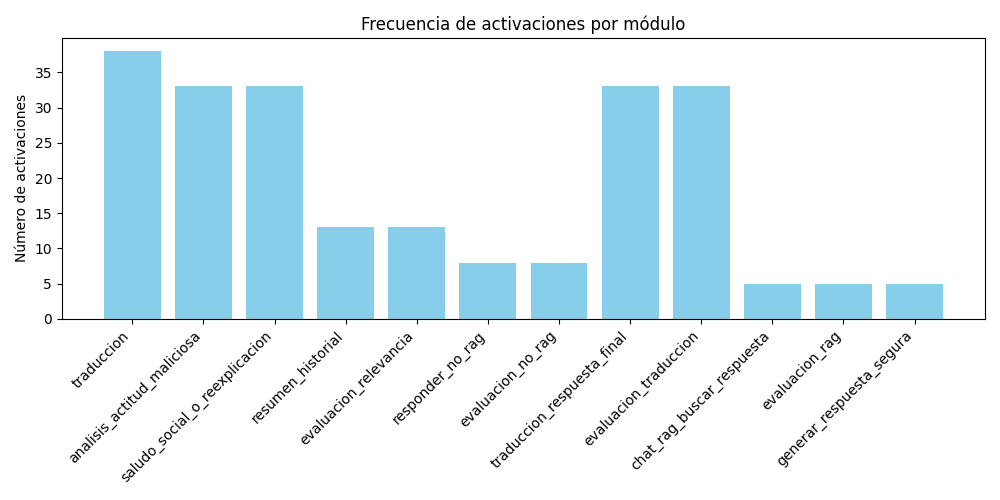
\includegraphics[width=0.9\textwidth]{../graficos/modulos_frecuencia.png}
\end{center}

\end{document}
